
\documentclass[11pt]{article}
\usepackage[margin=1in]{geometry}
\usepackage[T1]{fontenc}
\usepackage[utf8]{inputenc}
\usepackage{lmodern}
\usepackage{microtype}
\usepackage[table]{xcolor}
\usepackage{amsmath,amssymb,amsfonts,mathtools,bm}
\IfFileExists{physics.sty}{%
  \usepackage{physics}%
}{%
  % Portable subset used by this project when the optional physics package
  % is not installed in the local TeX distribution.
  \NewDocumentCommand{\pdv}{o m m}{%
    \IfNoValueTF{##1}{\frac{\partial ##2}{\partial ##3}}%
    {\frac{\partial^{##1} ##2}{\partial ##3^{##1}}}%
  }
  \NewDocumentCommand{\dv}{o m m}{%
    \IfNoValueTF{##1}{\frac{\mathrm{d} ##2}{\mathrm{d} ##3}}%
    {\frac{\mathrm{d}^{##1} ##2}{\mathrm{d} ##3^{##1}}}%
  }
  \providecommand{\dd}{\mathop{}\!\mathrm{d}}
  \providecommand{\grad}{\nabla}
  \providecommand{\abs}[1]{\left\lvert ##1\right\rvert}
  \providecommand{\norm}[1]{\left\lVert ##1\right\rVert}
  \providecommand{\ket}[1]{\left\lvert ##1\right\rangle}
  \providecommand{\bra}[1]{\left\langle ##1\right\rvert}
}
\usepackage{booktabs,array,longtable,tabularx}
\usepackage{hyperref}
\usepackage{enumitem}
\usepackage{fancyhdr}
\usepackage{titlesec}
\usepackage{tcolorbox}
\usepackage{ragged2e}
\usepackage{setspace}
\IfFileExists{siunitx.sty}{%
  \usepackage{siunitx}%
}{%
  % Minimal text-safe fallback for the small number of \SI and \si calls in
  % this repository. Full siunitx formatting is used when available.
  \providecommand{\si}[1]{\ensuremath{\mathrm{##1}}}
  \providecommand{\SI}[2]{\ensuremath{##1\,\mathrm{##2}}}
}
\hypersetup{colorlinks=true, linkcolor=blue!50!black, urlcolor=blue!50!black, citecolor=blue!50!black}
\definecolor{TitleBlue}{HTML}{163A5F}
\definecolor{AccentTeal}{HTML}{2D6F73}
\definecolor{SoftBlue}{HTML}{EAF3F8}
\definecolor{SoftTeal}{HTML}{EDF8F6}
\definecolor{SoftGray}{HTML}{F5F7FA}
\definecolor{RuleGray}{HTML}{D7DEE8}
\pagestyle{fancy}
\fancyhf{}
\lhead{RadiationEffects\_proj2}
\rhead{Technical Notes}
\cfoot{\thepage}
\setlength{\headheight}{14pt}
\setlength{\parskip}{0.5em}
\setlength{\parindent}{0pt}
\onehalfspacing
\numberwithin{equation}{section}
\titleformat{\section}{\Large\bfseries\color{TitleBlue}}{\thesection}{0.6em}{}
\titleformat{\subsection}{\large\bfseries\color{AccentTeal}}{\thesubsection}{0.6em}{}
\titleformat{\subsubsection}{\normalsize\bfseries\color{TitleBlue}}{\thesubsubsection}{0.6em}{}
\newtcolorbox{overviewbox}{colback=SoftBlue,colframe=TitleBlue,boxrule=0.8pt,arc=2mm,left=3mm,right=3mm,top=2mm,bottom=2mm}
\newtcolorbox{physicsbox}{colback=SoftTeal,colframe=AccentTeal,boxrule=0.8pt,arc=2mm,left=3mm,right=3mm,top=2mm,bottom=2mm}
\newtcolorbox{notebox}{colback=SoftGray,colframe=AccentTeal,boxrule=0.6pt,arc=2mm,left=3mm,right=3mm,top=2mm,bottom=2mm}
\newcommand{\DocTitle}[3]{%
\begin{center}
{\LARGE \bfseries \color{TitleBlue} #1}\\[0.5em]
{\large \color{AccentTeal} #2}\\[0.8em]
{\normalsize #3}
\end{center}
\vspace{0.5em}}
\newenvironment{symtable}{\rowcolors{2}{SoftGray}{white}\begin{longtable}{>{\RaggedRight\arraybackslash}p{0.18\textwidth} >{\RaggedRight\arraybackslash}p{0.25\textwidth} >{\RaggedRight\arraybackslash}p{0.47\textwidth}}\toprule \textbf{Symbol / acronym} & \textbf{Name} & \textbf{Meaning in this document} \\ \midrule\endfirsthead\toprule \textbf{Symbol / acronym} & \textbf{Name} & \textbf{Meaning in this document} \\ \midrule\endhead}{\bottomrule\end{longtable}}


\newcommand{\ProjectTOC}{%
\vspace{0.6em}
{\hypersetup{linkcolor=TitleBlue,urlcolor=TitleBlue,citecolor=TitleBlue}\tableofcontents}
\vspace{1.0em}}

\newcommand{\SymbolsAcronymsSection}{%
\section*{Symbols and acronyms used in this document}%
\addcontentsline{toc}{section}{Symbols and acronyms used in this document}}

\newcommand{\rvec}{\bm{r}}
\newcommand{\qvec}{\bm{q}}
\newcommand{\nvec}{\bm{n}}
\newcommand{\xvec}{\bm{x}}
\newcommand{\kB}{k_{\mathrm{B}}}
\newcommand{\qp}{\mathrm{qp}}
\newcommand{\JJ}{\mathrm{JJ}}
\newcommand{\mfp}{\Lambda}
\allowdisplaybreaks

\usepackage{tikz}
\usetikzlibrary{arrows.meta,positioning,shapes.geometric,calc}

\newcommand{\Cslow}{C}
\newcommand{\Ci}{C_i}
\newcommand{\Cj}{C_j}
\newcommand{\Dlat}{D}
\newcommand{\Dij}{D_i}
\newcommand{\Rrxn}{R}
\newcommand{\Gsrc}{G}
\newcommand{\Tfield}{T}
\newcommand{\Edep}{E_{\mathrm{dep}}}
\newcommand{\Edisp}{E_{\mathrm{d}}}
\newcommand{\Emig}{E_{\mathrm{m}}}
\newcommand{\Eann}{E_{\mathrm{ann}}}
\newcommand{\kann}{k_{\mathrm{ann}}}
\newcommand{\Om}{\Omega}
\newcommand{\Osub}{\Omega_{\mathrm{sub}}}
\newcommand{\Oox}{\Omega_{\mathrm{ox}}}
\newcommand{\Oint}{\Gamma_{\mathrm{int}}}
\newcommand{\Osc}{\Omega_{\mathrm{sc}}}
\newcommand{\Gam}{\Gamma}
\newcommand{\Jdef}{\mathbf{J}}
\newcommand{\nvecb}{\mathbf{n}}
\newcommand{\x}{\mathbf{x}}
\newcommand{\qpden}{n_{\mathrm{qp}}}
\newcommand{\Nph}{N_{\Omega}}
\newcommand{\DeltaSC}{\Delta}
\newcommand{\Tc}{T_{\mathrm{c}}}
\newcommand{\Tcr}{T_{\mathrm{c0}}}
\newcommand{\ellmfp}{\ell}
\newcommand{\xiSC}{\xi}
\newcommand{\lambdaL}{\lambda_{\mathrm{L}}}
\newcommand{\kBTe}{k_{\mathrm{B}}T}
\newcommand{\tauqp}{\tau_{\mathrm{qp}}}
\newcommand{\taur}{\tau_{\mathrm{r}}}
\newcommand{\tautrap}{\tau_{\mathrm{trap}}}
\newcommand{\Qoff}{Q_{\mathrm{off}}}
\newcommand{\rhoTrap}{\rho_{\mathrm{trap}}}
\newcommand{\phiEl}{\phi}
\newcommand{\muchem}{\mu}
\newcommand{\calM}{\mathcal{M}}
\newcommand{\calK}{\mathcal{K}}
\newcommand{\calR}{\mathcal{R}}
\newcommand{\wtest}{w}
\rhead{Module 3 Superconductivity Note}

\begin{document}

\DocTitle{Module 3 Superconductivity Extension: Defect Evolution in Cryogenic Superconducting-Device Materials}{Textbook-Style Physics Note for \texttt{RadiationEffects\_proj2}}{How the Module 3 defect diffusion-reaction model changes when the device is operated in a superconducting regime}

\hrule
\vspace{0.8em}

\begin{overviewbox}
\textbf{Purpose of this note.} The original Module 3 evolves radiation-induced defects in silicon using diffusion-reaction and annealing equations. This note derives how that picture must be modified for superconducting-device operation. The central correction is conceptual: at millikelvin or cryogenic temperatures, slow structural defects, trapped charges, interface two-level systems, nonequilibrium quasiparticles, and high-frequency phonons are not the same physical object. Module 3 should remain the structural and material-state evolution module, while passing fast superconducting excitations to Module 4 and Module 5. The superconducting extension therefore replaces the single warm-semiconductor defect picture with a material-resolved, timescale-separated model for substrate damage, oxide/interface traps, and superconducting-film disorder.
\end{overviewbox}

\ProjectTOC

\SymbolsAcronymsSection

\renewcommand{\arraystretch}{1.22}
\begin{longtable}{p{0.22\textwidth} p{0.55\textwidth} p{0.17\textwidth}}
\toprule
\textbf{Symbol / acronym} & \textbf{Meaning} & \textbf{Typical units} \\
\midrule
\endhead
$\Om$ & Full computational domain & m$^2$ or m$^3$ \\
$\Osub$ & Substrate domain, usually Si or sapphire in superconducting-chip context & m$^2$ or m$^3$ \\
$\Oox$ & Oxide or amorphous dielectric domain & m$^2$ or m$^3$ \\
$\Osc$ & Superconducting film domain, e.g. Al, Nb, Ta, TiN, NbTiN & m$^2$ or m$^3$ \\
$\Oint$ & Material interface, e.g. metal-oxide, oxide-substrate, metal-substrate & m or m$^2$ \\
$C_i(\x,t)$ & Concentration of structural defect species $i$ & m$^{-3}$ \\
$C_i^{(m)}$ & Concentration of defect species $i$ in material region $m$ & m$^{-3}$ \\
$C_{\mathrm{TLS}}$ & Areal or volumetric density of active two-level fluctuators & m$^{-2}$ or m$^{-3}$ \\
$f_a$ & Occupation probability of trap or TLS state $a$ & dimensionless \\
$\Jdef_i$ & Flux of defect species $i$ & m$^{-2}$ s$^{-1}$ \\
$D_i$ & Diffusivity of defect species $i$ & m$^2$/s \\
$D_{0,i}$ & Attempt-frequency diffusion prefactor & m$^2$/s \\
$E_{\mathrm{m},i}$ & Migration activation energy of defect species $i$ & eV or J \\
$G_i$ & Generation rate of defect species $i$ & m$^{-3}$ s$^{-1}$ \\
$R_i$ & Net reaction rate of defect species $i$ & m$^{-3}$ s$^{-1}$ \\
$k_{ij}$ & Reaction-rate coefficient coupling species $i$ and $j$ & problem-dependent \\
$T$ & Local temperature field & K \\
$T_{\mathrm{c}}$ & Local superconducting critical temperature & K \\
$\Delta$ & Superconducting energy gap & J or eV \\
$\Gamma$ & Pair-breaking or disorder-broadening parameter & J, eV, or s$^{-1}$ depending convention \\
$\ell$ & Electronic mean free path in the superconducting film & m \\
$\xi$ & Superconducting coherence length & m \\
$\lambda_{\mathrm{L}}$ & London penetration depth & m \\
$n_{\mathrm{qp}}$ & Nonequilibrium quasiparticle density & m$^{-3}$ \\
$N_{\Omega}$ & Population of phonons with energy above $2\Delta$ & m$^{-3}$ or mode count \\
$\tau_{\mathrm{r}}$ & Quasiparticle recombination time & s \\
$\tau_{\mathrm{trap}}$ & Quasiparticle trap or loss time & s \\
$Q_{\mathrm{off}}$ & Offset charge induced on a superconducting island & C \\
$\rho_{\mathrm{trap}}$ & Trapped charge density feeding Module 2 & C/m$^3$ \\
NIEL & Non-ionizing energy loss, energy partition relevant to displacement damage & eV/m or J/m \\
TLS & Two-level system, often defect-related fluctuator in amorphous or interfacial material & -- \\
QP & Quasiparticle, a broken-Cooper-pair excitation above the superconducting gap & -- \\
RT & Rothwarf-Taylor kinetic model for quasiparticle-phonon balance & -- \\
\bottomrule
\end{longtable}

\section{What Module 3 did before superconductivity}

In the original radiation-effects project, Module 3 receives an initial damage or defect-generation map from Module 1 and evolves that map in time. The baseline state variable is a concentration field,
\begin{equation}
C_i(x,y,t),
\end{equation}
for each defect species $i$. In the simplest one-species version, $C$ might represent an effective radiation-induced defect concentration. In a more detailed version, $C_i$ may represent vacancies, interstitials, vacancy-oxygen complexes, divacancies, charged traps, or other material defects.

The baseline governing equation is the diffusion-reaction balance law
\begin{equation}
\pdv{C_i}{t} + \nabla \cdot \Jdef_i = G_i + R_i,
\label{eq:baseline_balance}
\end{equation}
with Fickian flux
\begin{equation}
\Jdef_i = -D_i \nabla C_i.
\label{eq:fick}
\end{equation}
Substitution gives
\begin{equation}
\pdv{C_i}{t}=\nabla\cdot(D_i\nabla C_i)+G_i+R_i.
\label{eq:baseline_rd}
\end{equation}
The warm-semiconductor interpretation is straightforward. Radiation creates defects. Defects migrate by thermally activated hopping. Defects can recombine, cluster, dissociate, or anneal. The resulting defect field feeds Module 2 as charged space charge, Module 4 through heat-dependent rates, and Module 5 through recombination and trapping centers.

A common simplified annealing law is
\begin{equation}
R_i=-k_{\mathrm{ann},i} C_i,
\qquad
k_{\mathrm{ann},i}(T)=k_{0,i}\exp\left(-\frac{E_{\mathrm{ann},i}}{k_{\mathrm{B}}T}\right),
\label{eq:ann_law}
\end{equation}
and a common diffusion law is
\begin{equation}
D_i(T)=D_{0,i}\exp\left(-\frac{E_{\mathrm{m},i}}{k_{\mathrm{B}}T}\right).
\label{eq:arrheniusD}
\end{equation}
This is the correct starting point. The superconducting extension does not erase this logic. It changes the meaning of the state variables, the material regions, the active kinetic channels, and the coupling to the other modules.

\begin{physicsbox}
\textbf{Main transition from baseline Module 3 to superconducting Module 3.} The baseline model asks: how do radiation-induced lattice defects in silicon diffuse, react, and anneal? The superconducting extension asks: how do slow structural defects, trapped charges, interface fluctuators, superconducting-film disorder, and fast pair-breaking excitations evolve in a hybrid cryogenic superconducting device?
\end{physicsbox}

\section{What changes when the device enters the superconducting regime}

\subsection{The material is no longer a single silicon-like continuum}

A superconducting quantum device is usually not a block of superconducting silicon. A realistic device contains multiple material classes:
\begin{enumerate}[label=\arabic*.]
\item a crystalline substrate, often Si or sapphire,
\item native oxide or deposited dielectric layers,
\item metal-substrate and metal-oxide interfaces,
\item superconducting films and islands,
\item Josephson junction barriers, often thin amorphous oxides,
\item normal-metal traps, ground planes, packaging layers, and surface contamination.
\end{enumerate}

Therefore the defect state must become material-resolved. Instead of one concentration field $C_i(\x,t)$ on one domain, the natural superconducting-device state is
\begin{equation}
C_i^{(m)}(\x,t),
\qquad \x\in \Omega_m,
\label{eq:material_resolved_C}
\end{equation}
where $m$ labels the material region: substrate, oxide, interface, superconducting film, or junction barrier.


\begin{figure}[h]
\centering
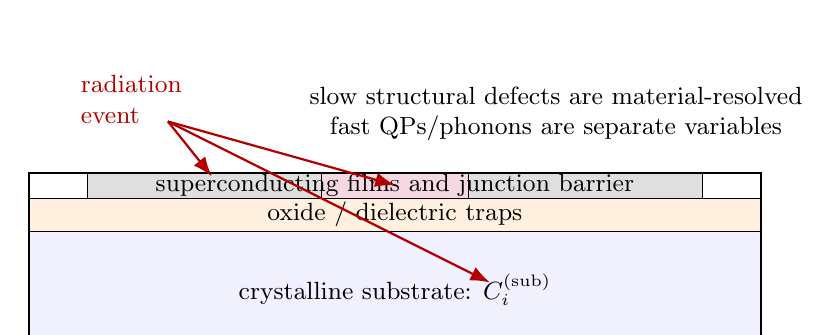
\begin{tikzpicture}[scale=0.93, every node/.style={font=\small}]
% layered stack
\fill[blue!6] (0,0) rectangle (10,1.55);
\fill[orange!12] (0,1.55) rectangle (10,2.0);
\fill[gray!25] (0.8,2.0) rectangle (4.0,2.35);
\fill[purple!15] (4.0,2.0) rectangle (6.0,2.35);
\fill[gray!25] (6.0,2.0) rectangle (9.2,2.35);
\draw[thick] (0,0) rectangle (10,2.35);
\draw (0,1.55) -- (10,1.55);
\draw (0,2.0) -- (10,2.0);
\draw (0.8,2.0) rectangle (4.0,2.35);
\draw (4.0,2.0) rectangle (6.0,2.35);
\draw (6.0,2.0) rectangle (9.2,2.35);
% internal labels
\node at (5,0.75) {crystalline substrate: $C_i^{(\mathrm{sub})}$};
\node at (5,1.78) {oxide / dielectric traps};
\node[align=center] at (5,2.18) {superconducting films and junction barrier};
% radiation event and explanatory label, placed outside the layer labels
\node[align=left,red!70!black] at (1.4,3.35) {radiation\\ event};
\draw[-{Latex[length=2.5mm]},thick,red!70!black] (1.9,3.05) -- (2.5,2.30);
\draw[-{Latex[length=2.5mm]},thick,red!70!black] (1.9,3.05) -- (5.0,2.18);
\draw[-{Latex[length=2.5mm]},thick,red!70!black] (1.9,3.05) -- (6.3,0.85);
\node[align=center] at (7.2,3.15) {slow structural defects are material-resolved\\ fast QPs/phonons are separate variables};
\end{tikzpicture}
\caption{A superconducting-device Module 3 model must be domain-aware. A radiation event can create substrate defects, oxide traps, interface fluctuators, and superconducting-film disorder. These are not identical species and they do not share the same mobility, reaction, or device impact.}
\label{fig:hybrid_domains_m3}
\end{figure}

\subsection{The temperature changes the kinetic hierarchy}

The most obvious change is that operation may occur at cryogenic or millikelvin temperature. But the consequence is not simply ``all defects stop.'' The correct statement is more precise:
\begin{itemize}
\item thermally activated migration of many atomic defects becomes exponentially suppressed;
\item ordinary thermal annealing becomes extremely slow;
\item radiation can still create defects nonthermally during the energy cascade;
\item electronic and phononic excitations can still move rapidly;
\item trapped charge and TLS occupation can fluctuate even when atoms do not diffuse appreciably;
\item local radiation hot spots can briefly raise the effective temperature enough to activate otherwise frozen channels.
\end{itemize}

The Arrhenius factor illustrates the scale. If $E_m=0.5\,\mathrm{eV}$, then at $T=300\,\mathrm{K}$,
\begin{equation}
\frac{E_m}{k_B T}\approx \frac{0.5}{0.0259}\approx 19.3,
\end{equation}
whereas at $T=0.1\,\mathrm{K}$,
\begin{equation}
\frac{E_m}{k_B T}\approx \frac{0.5}{8.62\times 10^{-6}\times 0.1}\approx 5.8\times 10^{5}.
\end{equation}
For a thermally activated jump, this is effectively frozen. Thus a cryogenic Module 3 model should usually treat structural diffusion as negligible between radiation events unless local heating or quantum-assisted tunneling is intentionally included.

\begin{notebox}
\textbf{Modeling consequence.} At cryogenic temperature, Module 3 may become less like a smooth long-time diffusion module and more like an event-driven damage-state update module: radiation deposits energy, creates structural defects and trapped charge, then most atomic defects remain nearly fixed while faster electronic, quasiparticle, and phonon variables relax through Modules 4 and 5.
\end{notebox}

\subsection{Superconductivity introduces new device sensitivities}

In a room-temperature semiconductor device, a defect matters mainly because it changes charge density, recombination, mobility, or leakage. In a superconducting circuit, a defect can matter through additional pathways:
\begin{enumerate}[label=\arabic*.]
\item it can trap charge and shift island offset charge;
\item it can behave as a TLS and absorb microwave energy;
\item it can locally suppress the superconducting gap $\Delta$;
\item it can reduce the electronic mean free path $\ell$;
\item it can increase kinetic inductance and surface resistance;
\item it can create quasiparticle traps or quasiparticle generation centers;
\item it can modify Josephson junction critical current through barrier disorder;
\item it can act as a magnetic or pair-breaking impurity.
\end{enumerate}

Therefore the output of Module 3 should no longer be only a charged-defect field. It should also supply local material parameters that feed superconducting models:
\begin{equation}
\{C_i^{(m)}\}\quad \longrightarrow \quad \rho_{\mathrm{trap}},\; C_{\mathrm{TLS}},\; \Delta(\x,t),\; T_c(\x,t),\; \ell(\x,t),\; D_{\mathrm{qp}}(\x,t),\; \tau_{\mathrm{trap}}(\x,t),\; I_c(\x,t).
\label{eq:defect_to_sc_parameters}
\end{equation}

\section{Timescale separation: structural defects are not quasiparticles}

\subsection{Slow variables and fast variables}

The first major error to avoid is to treat quasiparticles as ordinary lattice defects. A lattice defect is a structural imperfection: a vacancy, interstitial, impurity, complex, dislocation segment, oxide trap, or interface state. A quasiparticle is a broken-Cooper-pair excitation. It is an electronic excitation, not a missing atom.

For the superconducting extension, it is helpful to divide state variables into at least two classes:
\begin{align}
\text{slow structural/material state:} \qquad
& C_i^{(m)}(\x,t),\; C_{\mathrm{TLS}}(\x,t),\; f_a(\x,t), \label{eq:slow_vars}\\
\text{fast superconducting excitation state:} \qquad
& n_{\mathrm{qp}}(\x,t),\; N_{\Omega}(\x,t),\; T_{\mathrm{ph}}(\x,t),\; T_{\mathrm{e}}(\x,t). \label{eq:fast_vars}
\end{align}
The slow state belongs naturally to Module 3. The fast state overlaps more strongly with Module 4 and Module 5. Module 3 may store slowly evolving parameters that influence quasiparticle dynamics, but it should not confuse a transient quasiparticle burst with a permanent defect concentration.

\subsection{A mathematical expression of timescale separation}

Let $\tau_{\mathrm{def}}$ be the characteristic time for structural defect motion, and let $\tau_{\mathrm{qp}}$ be the quasiparticle relaxation time. A cryogenic superconducting-device model often has
\begin{equation}
\tau_{\mathrm{qp}} \ll \tau_{\mathrm{def}},
\end{equation}
although radiation-generated phonon and quasiparticle relaxation can still be long on qubit timescales. If the structural variables barely move during the fast relaxation of quasiparticles, then one can write
\begin{equation}
C_i^{(m)}(\x,t) \approx C_i^{(m)}(\x,t_0^+) \quad \text{for} \quad t_0<t<t_0+\tau_{\mathrm{qp}},
\label{eq:frozen_structural_during_qp}
\end{equation}
while $n_{\mathrm{qp}}$ and phonons evolve rapidly on that fixed damage landscape.

After the fast transient has ended, the slow defect state may be advanced by a larger time step, or it may simply be held fixed until the next radiation event if cryogenic diffusion is negligible.

\begin{physicsbox}
\textbf{Correct modeling split.} Module 3 should evolve the structural state that defines the material landscape. Module 4 should evolve heat and pair-breaking phonons. Module 5 should evolve carrier, trap, and quasiparticle populations. The superconducting Module 3 note therefore emphasizes which variables belong in Module 3 and which variables should be passed to the other modules.
\end{physicsbox}

\section{Material-resolved diffusion-reaction equations}

\subsection{General multispecies balance law}

For a material region $m$, let $C_i^{(m)}(\x,t)$ be the concentration of defect species $i$. The general balance law is
\begin{equation}
\pdv{C_i^{(m)}}{t}
=\nabla\cdot\left(D_i^{(m)}\nabla C_i^{(m)}\right)
+G_i^{(m)}
+R_i^{(m)}(\{C_j^{(m)}\},T,\phi,\Delta,\ldots).
\label{eq:material_rd}
\end{equation}
This is the direct superconducting-device generalization of the baseline Module 3 equation. The difference is that $m$ matters. A vacancy in crystalline silicon, a trap in amorphous oxide, and a disorder center in an aluminum film are different species living in different domains.

The diffusion coefficient is material-, species-, and temperature-dependent:
\begin{equation}
D_i^{(m)}(T)=D_{0,i}^{(m)}\exp\left(-\frac{E_{m,i}^{(m)}}{k_BT}\right),
\label{eq:mat_dep_diffusivity}
\end{equation}
with possible corrections for quantum tunneling, field-assisted motion, or local radiation heating.

The reaction term may include linear annealing, bimolecular recombination, clustering, and conversion among defect species:
\begin{equation}
R_i^{(m)}
= -k_{\mathrm{ann},i}^{(m)}C_i^{(m)}
-\sum_j k_{ij}^{(m)}C_i^{(m)}C_j^{(m)}
+\sum_{j,k} k_{jk\rightarrow i}^{(m)}C_j^{(m)}C_k^{(m)}
+\sum_j k_{j\rightarrow i}^{(m)}C_j^{(m)}
-\sum_j k_{i\rightarrow j}^{(m)}C_i^{(m)}.
\label{eq:general_reactions}
\end{equation}
This form is intentionally broad. In early versions of the code, only a few terms should be kept. The point of Eq.~\eqref{eq:general_reactions} is to show where the physical channels enter.

\subsection{Cryogenic freeze-out limit}

If $D_i^{(m)}\rightarrow 0$ and $k_{\mathrm{ann},i}^{(m)}\rightarrow 0$ at low temperature, the structural state equation reduces to
\begin{equation}
\pdv{C_i^{(m)}}{t}\approx G_i^{(m)}.
\label{eq:frozen_defect_eq}
\end{equation}
Between irradiation events, $G_i^{(m)}=0$, and therefore
\begin{equation}
C_i^{(m)}(\x,t)\approx \text{constant}.
\end{equation}
This is the frozen-defect approximation. It is not a claim that radiation has no effect at low temperature. It says the defect rearrangement after creation is suppressed.

\subsection{Event-update form}

For radiation-event modeling, it is often better to write Module 3 as a jump condition:
\begin{equation}
C_i^{(m)}(\x,t_k^+)=C_i^{(m)}(\x,t_k^-)+\Delta C_{i,k}^{(m)}(\x),
\label{eq:event_update}
\end{equation}
where $t_k$ is the time of radiation event $k$. The increment $\Delta C_{i,k}^{(m)}$ is obtained from Module 1 energy deposition and a defect-yield model. After the jump, the concentration may be evolved by Eq.~\eqref{eq:material_rd}; in the cryogenic freeze-out limit, that evolution is nearly static.

This event-update picture is often more faithful for superconducting quantum hardware than a smooth continuous damage-generation rate, because individual ionizing events can create burst-like disturbances.

\section{Radiation source terms at cryogenic temperature}

\subsection{Energy deposition is not equal to permanent defect production}

Module 1 gives an energy-deposition map. Not all deposited energy becomes permanent lattice damage. Energy can go into ionization, hot carriers, phonons, pair-breaking, local heating, scintillation-like channels, or displacement damage. Module 3 needs only the part that creates or transforms defects.

A useful general source model is
\begin{equation}
G_i^{(m)}(\x,t)
=\eta_i^{(m)}(T,\mathrm{particle},E)\frac{S_m(\x,t)}{E_{\mathrm{form},i}^{(m)}},
\label{eq:source_yield}
\end{equation}
where $S_m$ is the energy deposition rate density assigned to material region $m$, $E_{\mathrm{form},i}^{(m)}$ is an effective formation energy for defect species $i$, and $\eta_i^{(m)}$ is a yield factor. This equation is not a first-principles defect-production law; it is a controllable reduced model linking Module 1 output to Module 3 input.

For displacement damage, the more appropriate input is the non-ionizing part of the energy loss. A schematic NIEL-based form is
\begin{equation}
G_{\mathrm{disp}}^{(m)}(\x,t)
= \frac{\eta_{\mathrm{disp}}^{(m)}}{E_{\mathrm{d}}^{(m)}} S_{\mathrm{NIEL}}^{(m)}(\x,t),
\label{eq:niel_source}
\end{equation}
where $E_{\mathrm{d}}^{(m)}$ is an effective displacement threshold. This is closer to the physics of stable Frenkel-pair creation than using total deposited energy.

\subsection{Ionizing radiation can create traps without displacing atoms}

At cryogenic temperature, ionizing radiation can also change the charge state or occupation of preexisting traps. That is not the same as creating a new vacancy. Therefore a superconducting Module 3 should distinguish:
\begin{align}
\text{new structural defect creation:} &\qquad C_i \rightarrow C_i+\Delta C_i, \\
\text{trap charging or decharging:} &\qquad f_a \rightarrow f_a+\Delta f_a, \\
\text{quasiparticle creation:} &\qquad n_{\mathrm{qp}} \rightarrow n_{\mathrm{qp}}+\Delta n_{\mathrm{qp}}, \\
\text{phonon burst creation:} &\qquad N_{\Omega}\rightarrow N_{\Omega}+\Delta N_{\Omega}. 
\end{align}
The first belongs directly to Module 3. The second belongs to the interface/trap part of Module 3 and Module 2. The third and fourth should be passed primarily to Module 5 and Module 4.

\subsection{Partition of deposited energy}

A compact energy partition model is
\begin{equation}
S_{\mathrm{dep}}
=S_{\mathrm{ion}}+S_{\mathrm{disp}}+S_{\mathrm{ph}}+S_{\mathrm{qp}}+S_{\mathrm{heat}},
\label{eq:energy_partition}
\end{equation}
where only $S_{\mathrm{disp}}$ contributes directly to permanent displacement defects. In a superconducting film, $S_{\mathrm{qp}}$ may be significant because energy above $2\Delta$ can break Cooper pairs. But this produces quasiparticles, not structural defects. A structural defect model should therefore not use $S_{\mathrm{qp}}$ as if it were $S_{\mathrm{disp}}$.

\section{Cryogenic diffusion, annealing, and local hot spots}

\subsection{Arrhenius freeze-out derived from jump diffusion}

For a defect hopping between neighboring metastable sites separated by distance $a$, the jump rate is
\begin{equation}
\nu(T)=\nu_0\exp\left(-\frac{E_m}{k_BT}\right),
\label{eq:jump_rate}
\end{equation}
where $\nu_0$ is an attempt frequency. In $d$ dimensions, the diffusion coefficient scales as
\begin{equation}
D\sim \frac{a^2\nu}{2d}
=\frac{a^2\nu_0}{2d}\exp\left(-\frac{E_m}{k_BT}\right).
\label{eq:jump_diff}
\end{equation}
This gives the Arrhenius law in Eq.~\eqref{eq:mat_dep_diffusivity}. At millikelvin temperatures, $D$ becomes negligible for ordinary activated atomic migration.

\subsection{Radiation can create temporary local annealing windows}

Even if the bath temperature is $T_{\mathrm{bath}}\ll T_c$, a radiation event can produce a local transient temperature field $T(\x,t)$, or more precisely a nonequilibrium distribution of electronic and phonon energy. A reduced Module 3 model can represent this by using an effective local temperature in the rate constants:
\begin{equation}
D_i^{(m)}(\x,t)=D_{0,i}^{(m)}\exp\left[-\frac{E_{m,i}^{(m)}}{k_BT_{\mathrm{eff}}(\x,t)}\right].
\label{eq:TeffD}
\end{equation}
Then an otherwise frozen defect species can move only during a short hot window. If the hot window has duration $\delta t$, the mean squared diffusion length is approximately
\begin{equation}
\ell_{\mathrm{diff},i}^2\sim 2d\int_{t_k}^{t_k+\delta t}D_i(T_{\mathrm{eff}}(t))\,dt.
\label{eq:transient_diff_length}
\end{equation}
This equation is useful because it tells us when a complicated annealing model is unnecessary. If $\ell_{\mathrm{diff},i}$ is much smaller than the mesh size, then post-event diffusion is irrelevant at the resolved scale.

\subsection{Quantum tunneling of light defects}

Some light atoms or tunneling two-level systems may change state at cryogenic temperature through quantum tunneling rather than thermal activation. A phenomenological rate can be written
\begin{equation}
\gamma_a=\gamma_{a,0}\exp\left[-2\int_{x_1}^{x_2}\sqrt{\frac{2M_a(U_a(x)-E)}{\hbar^2}}\,dx\right],
\label{eq:wkb_tls_rate}
\end{equation}
which is the WKB transmission factor through a barrier. This form is relevant for TLS switching and local structural rearrangements in amorphous oxides. It is not usually the dominant mechanism for heavy lattice defects in crystalline silicon, but it is important conceptually because it explains why some low-temperature defect dynamics can remain active even when Arrhenius diffusion is frozen.

\section{Trapped charge and two-level systems at interfaces}

\subsection{Why interface defects matter more in superconducting devices}

In superconducting circuits, electric fields are concentrated near metal edges, thin oxides, junction barriers, and substrate-air or substrate-metal interfaces. Even a small density of defects in these regions can couple strongly to microwave modes or qubit island charge. Therefore the superconducting Module 3 model should treat interfaces as their own lower-dimensional defect domains.

Let $C_a^{(\Gamma)}(s,t)$ be the areal density of interface defect type $a$ along interface coordinate $s$. A surface balance law is
\begin{equation}
\pdv{C_a^{(\Gamma)}}{t}
=\nabla_s\cdot\left(D_a^{(\Gamma)}\nabla_s C_a^{(\Gamma)}\right)
+G_a^{(\Gamma)}+R_a^{(\Gamma)},
\label{eq:surface_defect_balance}
\end{equation}
where $\nabla_s$ is the surface gradient. At cryogenic temperature, the diffusion term may again vanish, but the generation and occupation terms can remain important.

\subsection{Trap occupation kinetics}

A trap density and a trap occupation are different quantities. The total number of available traps may be $C_a$, while the occupied fraction is $f_a$. A minimal kinetic equation for occupation is
\begin{equation}
\pdv{f_a}{t}=\gamma_{a}^{+}(1-f_a)-\gamma_a^{-}f_a,
\label{eq:trap_occupation}
\end{equation}
where $\gamma_a^+$ is the capture or charging rate and $\gamma_a^-$ is the emission or decharging rate. The trapped charge density entering Module 2 is then
\begin{equation}
\rho_{\mathrm{trap}}(\x,t)=\sum_a q_a C_a(\x,t) f_a(\x,t).
\label{eq:trap_charge_density}
\end{equation}
This equation is important. It separates the structural existence of a trap from its instantaneous charge state. Radiation may change either one.

\subsection{Two-level fluctuator model}

A TLS can be represented as a local degree of freedom with two metastable configurations. A simple classical occupation variable $p_a$ obeys
\begin{equation}
\pdv{p_a}{t}=\gamma_{a,1\rightarrow2}(1-p_a)-\gamma_{a,2\rightarrow1}p_a.
\label{eq:tls_rate}
\end{equation}
The TLS contributes to dielectric loss or charge noise through its dipole moment, charge state, or local polarizability. The structural density of active TLSs belongs to Module 3; their electromagnetic coupling is used in Module 2 and later device-response modules.

If a TLS has electric dipole moment $\mathbf{p}_a$, its coupling energy to a local electric field is
\begin{equation}
U_a=-\mathbf{p}_a\cdot \mathbf{E}(\x_a),
\label{eq:tls_coupling}
\end{equation}
where $\mathbf{E}$ comes from Module 2. This is one reason Module 2 and Module 3 become tightly coupled in superconducting devices.

\section{Defects inside superconducting films}

\subsection{Structural disorder and electronic mean free path}

In a superconducting metal film, structural defects affect the normal-state scattering rate. A simple Matthiessen-like model is
\begin{equation}
\frac{1}{\ell(\x,t)}
=\frac{1}{\ell_0}+\sum_i \sigma_i C_i^{(\mathrm{sc})}(\x,t),
\label{eq:mfp_defects}
\end{equation}
where $\ell_0$ is the pre-irradiation mean free path and $\sigma_i$ is an effective scattering cross section for defect species $i$. The normal-state electronic diffusion constant is approximately
\begin{equation}
D_N(\x,t)=\frac{1}{3}v_F\ell(\x,t)
\label{eq:DN_mfp}
\end{equation}
for an isotropic metal.

The quasiparticle diffusion coefficient used later in Module 5 is related to this normal diffusion constant, often with energy- and gap-dependent corrections. Thus Module 3 influences quasiparticle spreading by changing $\ell$ and $D_N$.

\subsection{Dirty-limit superconducting length scales}

In the dirty limit, where $\ell$ is shorter than the clean coherence length, a useful scale for the coherence length is
\begin{equation}
\xi_{\mathrm{dirty}}\sim \sqrt{\frac{\hbar D_N}{\Delta}}.
\label{eq:dirty_xi}
\end{equation}
This equation shows how structural disorder enters superconducting electrodynamics. More defects reduce $\ell$, which reduces $D_N$, which changes $\xi$. The London penetration depth and kinetic inductance can also increase with disorder. A common phenomenological trend is
\begin{equation}
\lambda_{\mathrm{eff}}(\x,t)=\lambda_{\mathrm{L0}}\,F_{\lambda}(\ell(\x,t),\Delta(\x,t),T),
\label{eq:lambda_eff}
\end{equation}
with $F_{\lambda}>1$ in disordered thin films. The exact form depends on material and regime, so Eq.~\eqref{eq:lambda_eff} should initially be implemented phenomenologically rather than overfit.

\subsection{Critical temperature and superconducting gap suppression}

The superconducting transition temperature and gap can be modified by disorder, impurities, magnetic moments, oxide contamination, film morphology, and radiation-induced damage. A linear reduced model is
\begin{equation}
T_c(\x,t)=T_{c0}-\sum_i a_i C_i^{(\mathrm{sc})}(\x,t),
\label{eq:Tc_linear_damage}
\end{equation}
with the constraint $T_c\ge 0$. This is not universal, but it is a practical first model.

For conventional $s$-wave superconductors, nonmagnetic disorder does not necessarily suppress $T_c$ strongly in the ideal Anderson-theorem limit. But real films are finite, oxidized, granular, strained, and sometimes close to localization or pair-breaking regimes. Therefore a local damage-to-$T_c$ relation should be treated as material-dependent.

For magnetic or pair-breaking impurities, a more microscopic reference form is the Abrikosov-Gorkov-type relation
\begin{equation}
\ln\left(\frac{T_{c0}}{T_c}\right)
=\psi\left(\frac{1}{2}+\frac{\Gamma}{2\pi k_B T_c}\right)-\psi\left(\frac{1}{2}\right),
\label{eq:ag}
\end{equation}
where $\psi$ is the digamma function and $\Gamma$ is a pair-breaking parameter. Module 3 can connect this to defects through
\begin{equation}
\Gamma(\x,t)=\Gamma_0+\sum_i g_i C_i^{(\mathrm{sc})}(\x,t).
\label{eq:gamma_defects}
\end{equation}
This is a clearer physics pathway than saying vaguely that defects degrade superconductivity.

\subsection{Gap inhomogeneity as a Module 3 output}

A useful superconducting extension output is a local gap map:
\begin{equation}
\Delta(\x,t)=\Delta_0\,F_{\Delta}(T,T_c(\x,t),\Gamma(\x,t),\{C_i^{(\mathrm{sc})}\}).
\label{eq:gap_map_general}
\end{equation}
For weak-coupling BCS at low pair-breaking and uniform material,
\begin{equation}
\Delta(0)\approx 1.764\,k_BT_c,
\label{eq:bcs_gap}
\end{equation}
but in an irradiated thin film this should be treated as a baseline relation, not a law that captures all morphology and disorder effects.

This gap map is crucial because phonons with energy $\hbar\omega>2\Delta$ can break Cooper pairs, while phonons below that threshold cannot directly create quasiparticles through pair breaking. Therefore Module 3 defect-induced changes in $\Delta$ affect Module 4 phonon downconversion and Module 5 quasiparticle generation.

\section{Josephson junction barrier defects}

\subsection{Junction barriers are special material domains}

A Josephson junction barrier is typically extremely thin, often an amorphous oxide. Its defects can strongly affect critical current, charge noise, TLS loss, and junction asymmetry. In a simplified transmon-level model, the Josephson energy is
\begin{equation}
E_J=\frac{\hbar I_c}{2e}.
\label{eq:EJ_Ic}
\end{equation}
A change in barrier defect state can therefore change $I_c$ and shift the qubit frequency.

A phenomenological defect-to-critical-current relation is
\begin{equation}
I_c(t)=I_{c0}\exp\left[-\int_{\Omega_{\mathrm{JJ}}}\sum_i b_i C_i^{(\mathrm{JJ})}(\x,t)\,d\ell\right],
\label{eq:Ic_barrier_defects}
\end{equation}
where $\Omega_{\mathrm{JJ}}$ denotes the barrier region and $b_i$ are sensitivity coefficients. The exponential form is natural because tunneling through a barrier is exponentially sensitive to barrier height and thickness, although the exact coefficients are device-specific.

\subsection{TLS density in the junction barrier}

If the junction barrier contains active TLSs, their density may be evolved as
\begin{equation}
\pdv{C_{\mathrm{TLS}}^{(\mathrm{JJ})}}{t}
=G_{\mathrm{TLS}}^{(\mathrm{JJ})}-k_{\mathrm{relax}} C_{\mathrm{TLS}}^{(\mathrm{JJ})},
\label{eq:jj_tls_evolution}
\end{equation}
where $G_{\mathrm{TLS}}$ represents radiation activation or creation of fluctuators, and $k_{\mathrm{relax}}$ represents slow relaxation or annealing. At millikelvin temperatures $k_{\mathrm{relax}}$ may be very small unless the device is warmed up.

\section{Quasiparticles and pair-breaking phonons: auxiliary, not structural, species}

\subsection{Minimal quasiparticle continuity equation}

Although quasiparticles should not be treated as permanent defects, Module 3 must know how its structural state influences them. The local quasiparticle density can be modeled by
\begin{equation}
\pdv{n_{\mathrm{qp}}}{t}
=\nabla\cdot\left(D_{\mathrm{qp}}\nabla n_{\mathrm{qp}}\right)
+G_{\mathrm{pb}}
-R_{\mathrm{rec}}(n_{\mathrm{qp}})
-R_{\mathrm{trap}}(n_{\mathrm{qp}}),
\label{eq:qp_diffusion_reaction}
\end{equation}
where $G_{\mathrm{pb}}$ is pair-breaking generation, $R_{\mathrm{rec}}$ is recombination, and $R_{\mathrm{trap}}$ is trapping or loss. This equation belongs mainly to Module 5, but its coefficients depend on Module 3:
\begin{equation}
D_{\mathrm{qp}}=D_{\mathrm{qp}}(\ell,\Delta,T),
\qquad
\tau_{\mathrm{trap}}=\tau_{\mathrm{trap}}(C_{\mathrm{trap}},\Delta,\mathrm{geometry}).
\label{eq:qp_coeffs_from_m3}
\end{equation}

\subsection{Rothwarf-Taylor form}

A compact quasiparticle-phonon kinetic model is the Rothwarf-Taylor form:
\begin{align}
\dv{N_{\mathrm{qp}}}{t}
&= -R\,N_{\mathrm{qp}}^2 + 2\beta N_{\Omega}+G_{\mathrm{qp}}-\frac{N_{\mathrm{qp}}}{\tau_{\mathrm{trap}}},
\label{eq:rt_qp}\\
\dv{N_{\Omega}}{t}
&= \frac{1}{2}R\,N_{\mathrm{qp}}^2 - \beta N_{\Omega}-\frac{N_{\Omega}}{\tau_{\mathrm{esc}}}+G_{\Omega}.
\label{eq:rt_ph}
\end{align}
Here $N_{\Omega}$ denotes phonons energetic enough to break Cooper pairs. $R$ is a recombination coefficient, and $\beta$ is a pair-breaking coefficient. The factor of 2 in Eq.~\eqref{eq:rt_qp} reflects that one pair-breaking phonon creates two quasiparticles.

This model should be referenced in Module 3 but probably implemented in Module 5 or in the coupled Module 6 loop. Module 3 supplies structural parameters that affect $R$, $\beta$, $\tau_{\mathrm{trap}}$, and $\tau_{\mathrm{esc}}$.

\begin{notebox}
\textbf{Important naming rule.} In the code, avoid naming $n_{\mathrm{qp}}$ as \texttt{defectConcentration}. Use names like \texttt{qpDensity}, \texttt{pairBreakingPhononDensity}, or \texttt{fastExcitationState}. This prevents a serious physics confusion between structural damage and superconducting excitations.
\end{notebox}

\section{Deriving the superconducting Module 3 state vector}

\subsection{Baseline vector}

The baseline Module 3 state could be represented as
\begin{equation}
\mathbf{u}_{3}=\begin{bmatrix}
C_1 \\ C_2 \\ \vdots \\ C_N
\end{bmatrix}.
\label{eq:baseline_state_vector}
\end{equation}
For a semiconductor-only model, this may be enough.

\subsection{Superconducting-device state vector}

For the superconducting extension, a better state vector is
\begin{equation}
\mathbf{u}_{3}^{\mathrm{SC}}
=\left[
\begin{array}{c}
\{C_i^{(\mathrm{sub})}\}\\
\{C_i^{(\mathrm{ox})}\}\\
\{C_i^{(\Gamma)}\}\\
\{f_a^{(\Gamma)}\}\\
\{C_i^{(\mathrm{sc})}\}\\
\{C_i^{(\mathrm{JJ})}\}
\end{array}
\right].
\label{eq:sc_state_vector}
\end{equation}
The quasiparticle density is intentionally not included as a structural defect species. Instead, Module 3 produces a parameter map
\begin{equation}
\mathbf{p}_{\mathrm{SC}}[\mathbf{u}_{3}^{\mathrm{SC}}]
=\{\rho_{\mathrm{trap}},C_{\mathrm{TLS}},\ell,D_N,D_{\mathrm{qp}},\Delta,T_c,\tau_{\mathrm{trap}},I_c\}.
\label{eq:parameter_output}
\end{equation}
This parameter map is the bridge from defect evolution to superconducting-device performance.

\section{Coupling to Module 2: charged defects, trapped charge, and offset charge}

Module 2 solves electrostatics. In a superconducting device, the most important Module 3 outputs for Module 2 are charged defects and trap occupations. From Eq.~\eqref{eq:trap_charge_density}, the charge density is
\begin{equation}
\rho_{\mathrm{def+trap}}(\x,t)=\sum_i q_i C_i(\x,t)+\sum_a q_a C_a(\x,t) f_a(\x,t).
\label{eq:rho_def_trap_m3}
\end{equation}
This charge density then enters the Poisson or screened-Poisson model of Module 2.

For a superconducting island, the important quantity is often not the full local charge map but the induced offset charge:
\begin{equation}
Q_{\mathrm{off}}(t)=\int_{\Omega_{\mathrm{dielectric}}} \rho_{\mathrm{trap}}(\x,t)\,\psi(\x)\,d\Omega,
\label{eq:qoff_weighting}
\end{equation}
where $\psi(\x)$ is a weighting potential determined by the island geometry. Module 3 supplies $\rho_{\mathrm{trap}}$; Module 2 supplies $\psi$.

A trap switching event changes the offset charge by
\begin{equation}
\Delta Q_{\mathrm{off},a}=q_a\,\Delta f_a\,\psi(\x_a).
\label{eq:qoff_jump}
\end{equation}
This is the mathematical link between a microscopic defect occupation change and a macroscopic superconducting qubit charge offset.

\section{Coupling to Module 4: temperature, phonons, and local heating}

Module 4 controls thermal and phonon physics. It feeds Module 3 through temperature-dependent rates:
\begin{equation}
D_i=D_i(T),\qquad k_i=k_i(T),\qquad \gamma_a=\gamma_a(T,E,\mathrm{strain}).
\label{eq:m4_to_m3_rates}
\end{equation}
At ordinary cryogenic bath temperature, these rates may be nearly zero. But after an irradiation event, Module 4 may predict a transient hot phonon or local temperature field. Module 3 should then integrate the rates over the transient window, as in Eq.~\eqref{eq:transient_diff_length}.

Module 3 feeds Module 4 by changing phonon scattering and downconversion properties. A defect-rich region may scatter phonons more strongly:
\begin{equation}
\frac{1}{\tau_{\mathrm{ph}}(\omega,\x,t)}
=\frac{1}{\tau_{\mathrm{ph},0}(\omega)}+
\sum_i A_i(\omega) C_i(\x,t).
\label{eq:phonon_scattering_defects}
\end{equation}
This affects whether high-energy phonons propagate far enough to break Cooper pairs in distant superconducting regions.

\section{Coupling to Module 5: traps, recombination, and quasiparticle poisoning}

Module 5 originally describes carrier drift-diffusion and recombination. In the superconducting extension, it must also eventually describe quasiparticle generation, diffusion, recombination, and trapping. Module 3 provides the structural parameters needed for these processes:
\begin{align}
\tau_{\mathrm{trap}}^{-1}(\x,t)&=\tau_{\mathrm{trap},0}^{-1}+\sum_i s_i C_i^{(\mathrm{sc})}(\x,t),
\label{eq:trap_rate_defect}\\
R_{\mathrm{rec}}(\x,t)&=R_0\,F_R(\Delta(\x,t),T,\mathrm{disorder}),
\label{eq:recomb_defect}\\
D_{\mathrm{qp}}(\x,t)&=D_{\mathrm{qp}}(\ell(\x,t),\Delta(\x,t),T).
\label{eq:Dqp_defect}
\end{align}
These equations do not require Module 3 to solve quasiparticle dynamics. They require Module 3 to output the defect-dependent material landscape on which quasiparticles evolve.

\section{Boundary and interface conditions}

\subsection{No-flux boundaries for frozen structural defects}

At external boundaries where defects cannot leave the computational domain, use
\begin{equation}
\nvecb\cdot \Jdef_i=0,
\qquad
\text{or}
\qquad
\nvecb\cdot D_i\nabla C_i=0.
\label{eq:no_flux}
\end{equation}
This is the standard Neumann no-flux condition.

\subsection{Interface transfer between regions}

If a defect species can cross from material $a$ to material $b$, continuity of flux requires
\begin{equation}
\nvecb_a\cdot \Jdef_i^{(a)}=-\nvecb_b\cdot \Jdef_i^{(b)}.
\label{eq:flux_continuity}
\end{equation}
The concentrations themselves need not be continuous if the defect has different formation energies in the two materials. A thermodynamic partition relation can be written
\begin{equation}
C_i^{(b)}=K_{ab,i} C_i^{(a)},
\label{eq:partition_condition}
\end{equation}
where $K_{ab,i}$ is a segregation coefficient.

At cryogenic temperature, many structural species will not cross interfaces at all, and Eq.~\eqref{eq:no_flux} may be appropriate. But for hydrogen, oxygen-related species, charge states, or interface traps, special transfer or trapping conditions may be needed.

\subsection{Surface trap generation}

Radiation or phonons can activate surface traps. A surface source condition can be written
\begin{equation}
-D_i\nabla C_i\cdot \nvecb = S_{\Gamma,i} - k_{\Gamma,i} C_i,
\label{eq:surface_source_sink}
\end{equation}
where $S_{\Gamma,i}$ is surface defect generation or activation and $k_{\Gamma,i}$ is a surface sink rate. This Robin-type condition is useful for interfaces where the surface is not merely reflecting.

\section{Finite-element weak form for superconducting Module 3}

\subsection{Weak form for one material region}

Start from
\begin{equation}
\pdv{C_i}{t}=\nabla\cdot(D_i\nabla C_i)+G_i+R_i.
\end{equation}
Multiply by a test function $w$ and integrate over a region $\Omega_m$:
\begin{equation}
\int_{\Omega_m} w\pdv{C_i}{t}\,d\Omega
=\int_{\Omega_m} w\nabla\cdot(D_i\nabla C_i)\,d\Omega
+\int_{\Omega_m} w(G_i+R_i)\,d\Omega.
\end{equation}
Integrating the diffusion term by parts gives
\begin{equation}
\int_{\Omega_m} w\pdv{C_i}{t}\,d\Omega
+\int_{\Omega_m}\nabla w\cdot D_i\nabla C_i\,d\Omega
=\int_{\Omega_m} w(G_i+R_i)\,d\Omega
+\int_{\partial\Omega_m} w D_i\nabla C_i\cdot \nvecb\,d\Gamma.
\label{eq:weak_m3_sc}
\end{equation}
This is the FEM weak form. For no-flux boundaries, the boundary integral vanishes. For surface generation or trapping, Eq.~\eqref{eq:surface_source_sink} supplies the boundary term.

\subsection{Discrete matrix form}

Approximate
\begin{equation}
C_i(\x,t)=\sum_a N_a(\x) C_{i,a}(t),
\qquad
w=N_b.
\end{equation}
The mass matrix and diffusion matrix are
\begin{align}
M_{ba}^{(m)}&=\int_{\Omega_m} N_b N_a\,d\Omega,\\
K_{ba}^{(m)}&=\int_{\Omega_m} \nabla N_b\cdot D_i^{(m)}\nabla N_a\,d\Omega.
\end{align}
The semidiscrete equation is
\begin{equation}
\mathbf{M}^{(m)}\dot{\mathbf{C}}_i^{(m)}+
\mathbf{K}_i^{(m)}\mathbf{C}_i^{(m)}
=\mathbf{G}_i^{(m)}+\mathbf{R}_i^{(m)}+\mathbf{B}_i^{(m)}.
\label{eq:semi_discrete_m3_sc}
\end{equation}
For cryogenic freeze-out, $D_i^{(m)}\approx 0$, so the diffusion matrix may vanish. The remaining problem is local generation and reaction.

\subsection{Implicit Euler update}

For linear reaction $R_i=-k_iC_i$, an implicit Euler update is
\begin{equation}
\left[\mathbf{M}+\Delta t\left(\mathbf{K}+\mathbf{K}_{R}\right)\right]\mathbf{C}^{n+1}
=\mathbf{M}\mathbf{C}^{n}+\Delta t\left(\mathbf{G}^{n+1}+\mathbf{B}^{n+1}\right).
\label{eq:implicit_euler_m3_sc}
\end{equation}
At very low temperature, if $\mathbf{K}$ and $\mathbf{K}_R$ are negligible between events, this reduces to
\begin{equation}
\mathbf{C}^{n+1}\approx \mathbf{C}^{n}+\Delta t\,\mathbf{M}^{-1}\mathbf{G}^{n+1},
\end{equation}
or to the event update in Eq.~\eqref{eq:event_update}.

\section{Reduced model hierarchy for implementation}

\subsection{Level 0: frozen structural damage plus trap charge}

The minimal useful superconducting Module 3 extension is:
\begin{align}
C_i^{(m)}(t_k^+)&=C_i^{(m)}(t_k^-)+\Delta C_{i,k}^{(m)},\\
f_a(t_k^+)&=f_a(t_k^-)+\Delta f_{a,k},\\
C_i^{(m)}(t)&\approx \mathrm{constant}\quad \text{between events}.
\end{align}
Outputs:
\begin{equation}
\rho_{\mathrm{trap}},\quad Q_{\mathrm{off}},\quad C_{\mathrm{TLS}},\quad \Delta C_{\mathrm{damage}}.
\end{equation}
This is the most robust starting point.

\subsection{Level 1: transient local heating activates diffusion or annealing}

Add Module 4 temperature input:
\begin{equation}
D_i(\x,t)=D_i(T_{\mathrm{eff}}(\x,t)),
\qquad
k_i(\x,t)=k_i(T_{\mathrm{eff}}(\x,t)).
\end{equation}
Evolve Eq.~\eqref{eq:material_rd} only during and after thermal transients. This allows radiation hot spots to modify defect state even when the bath is cold.

\subsection{Level 2: superconducting material-parameter maps}

Add maps:
\begin{equation}
\ell(\x,t),\quad T_c(\x,t),\quad \Delta(\x,t),\quad D_{\mathrm{qp}}(\x,t),\quad \tau_{\mathrm{trap}}(\x,t),\quad I_c(t).
\end{equation}
These maps allow Module 5 and the final device-response module to predict quasiparticle poisoning, microwave loss, junction shifts, and kinetic-inductance changes.

\subsection{Level 3: coupled structural-excitation dynamics}

In the most complete model, structural defects, trap occupation, phonons, and quasiparticles are evolved together. The coupled state could be
\begin{equation}
\mathbf{u}_{\mathrm{coupled}}=\{C_i^{(m)},f_a,n_{\mathrm{qp}},N_{\Omega},T_{\mathrm{ph}},T_e,\phi\}.
\end{equation}
This belongs to Module 6 rather than Module 3 alone. Module 3 should remain clear about which parts of this state are structural.

\section{PINN and CPINN implications}

If a PINN or CPINN is later added to superconducting Module 3, the physics residual cannot simply copy the warm-semiconductor equation. It must include material labels, frozen coefficients, interface terms, and event ordering.

A PINN residual for structural species $i$ in material $m$ is
\begin{equation}
\mathcal{R}_{i}^{(m)}
=\pdv{C_i^{(m)}}{t}
-\nabla\cdot\left(D_i^{(m)}\nabla C_i^{(m)}\right)
-G_i^{(m)}-R_i^{(m)}.
\label{eq:pinn_residual_m3_sc}
\end{equation}
The loss can be written
\begin{equation}
\mathcal{L}_{\mathrm{M3SC}}
=\sum_{m,i}\lambda_{i,m}^{\mathrm{res}}\norm{\mathcal{R}_{i}^{(m)}}_2^2
+\lambda_{\Gamma}\mathcal{L}_{\Gamma}
+\lambda_{\mathrm{data}}\mathcal{L}_{\mathrm{data}}
+\lambda_{\mathrm{event}}\mathcal{L}_{\mathrm{event}}.
\label{eq:pinn_loss_m3_sc}
\end{equation}
For a CPINN, the natural causal ordering is not spatial. It is event, dose, or thermal-history ordering:
\begin{equation}
\{t_1<t_2<\cdots<t_K\}\quad \text{or}\quad \{\mathrm{dose}_1<\mathrm{dose}_2<\cdots<\mathrm{dose}_K\}.
\end{equation}
This is physically stronger for Module 3 than for Module 2, because Module 3 is genuinely time-evolutionary.

A causal weight for stage $k$ may be
\begin{equation}
w_k=\exp\left[-\epsilon\sum_{j<k}\mathcal{L}_j\right],
\label{eq:causal_weight_m3}
\end{equation}
where $\mathcal{L}_j$ is the residual and constraint loss at earlier stages. This prevents the network from fitting late-time or high-dose states before it has learned early damage generation and early relaxation.

\section{Verification tests for Module 3 superconductivity}

\subsection{Test 1: cryogenic freeze-out}

Set $G=0$, $D\approx0$, and $R\approx0$. The code should preserve the initial defect concentration:
\begin{equation}
C(\x,t)=C(\x,0).
\end{equation}
Any drift indicates numerical diffusion or unintended reaction terms.

\subsection{Test 2: event jump only}

Apply one radiation event with known $\Delta C(\x)$. The result should satisfy
\begin{equation}
C(\x,t^+)-C(\x,t^-)=\Delta C(\x).
\end{equation}
This tests the event-update interface from Module 1 to Module 3.

\subsection{Test 3: transient heating diffusion length}

Apply a prescribed temperature pulse $T(t)$ and compare the simulated broadening of a Gaussian defect packet with
\begin{equation}
\sigma^2(t)-\sigma^2(0)=2d\int_0^t D(T(t'))\,dt'.
\end{equation}
This tests the Arrhenius-rate coupling to Module 4.

\subsection{Test 4: trapped-charge offset}

Place a single charged trap at position $\x_a$ and compare the computed offset-charge jump with
\begin{equation}
\Delta Q_{\mathrm{off},a}=q_a\Delta f_a\psi(\x_a).
\end{equation}
This verifies the coupling between Module 3 trap occupation and Module 2 weighting potential.

\subsection{Test 5: disorder-to-gap map}

Use a uniform defect concentration in the superconducting film and verify that the generated maps $\ell(\x)$, $T_c(\x)$, and $\Delta(\x)$ remain uniform and follow the specified parameter laws. This checks that material-parameter outputs are deterministic and dimensionally consistent.

\section{Recommended first implementation for the project}

For \texttt{RadiationEffects\_proj2}, the best first superconducting Module 3 implementation should not attempt full microscopic superconducting kinetics. The most useful first version is:
\begin{enumerate}[label=\arabic*.]
\item keep the existing diffusion-reaction solver for compatibility;
\item add a \texttt{materialRegion} label for substrate, oxide/interface, superconducting film, and junction barrier;
\item add cryogenic Arrhenius freeze-out for diffusion and annealing;
\item add event-based defect increments from Module 1;
\item add trap occupation variables $f_a$;
\item output $\rho_{\mathrm{trap}}$ and $Q_{\mathrm{off}}$ for Module 2;
\item output phenomenological maps $\ell$, $\Delta$, $T_c$, $D_{\mathrm{qp}}$, and $\tau_{\mathrm{trap}}$ for Modules 4 and 5;
\item keep $n_{\mathrm{qp}}$ out of the structural defect array.
\end{enumerate}

This gives a physically defensible path without pretending to solve every microscopic problem at once.


\section{Charge-state kinetics of defects at low temperature}

\subsection{Structural concentration versus charge state}

A defect can exist structurally while its charge state changes. For defect type $i$, let $C_i$ be the total structural concentration and let $f_{i,q}$ be the fraction in charge state $q$. Then
\begin{equation}
C_{i,q}(\x,t)=C_i(\x,t)f_{i,q}(\x,t),
\qquad
\sum_q f_{i,q}=1.
\label{eq:charge_state_fraction}
\end{equation}
The charge density contributed by this defect is
\begin{equation}
\rho_i(\x,t)=\sum_q q e\,C_i(\x,t)f_{i,q}(\x,t).
\label{eq:defect_charge_states}
\end{equation}
At cryogenic temperature, $C_i$ may be frozen while $f_{i,q}$ changes due to ionization, tunneling, capture, emission, or radiation-induced charge rearrangement. This is another reason Module 3 should not only store a scalar defect density.

A minimal charge-state rate equation is
\begin{equation}
\pdv{f_{i,q}}{t}
=\sum_{q'\neq q}\gamma_{q'\rightarrow q}f_{i,q'}
-f_{i,q}\sum_{q'\neq q}\gamma_{q\rightarrow q'}.
\label{eq:charge_state_master}
\end{equation}
The transition rates may depend on local potential, electric field, radiation excitation, phonon bath, and quasiparticle density:
\begin{equation}
\gamma_{q\rightarrow q'}=
\gamma_{q\rightarrow q'}(\phi,\mathbf{E},T_{\mathrm{ph}},n_{\mathrm{qp}},S_{\mathrm{ion}}).
\end{equation}
This gives a precise interface between Module 3 trap states and Module 2 electrostatics.

\subsection{Detailed balance limit}

If the trap is in thermal equilibrium with a carrier reservoir at chemical potential $\mu$, a two-state trap with energy $E_t$ has the equilibrium occupation
\begin{equation}
f_t^{\mathrm{eq}}=\frac{1}{1+\exp[(E_t-\mu)/k_BT]}.
\label{eq:trap_fermi}
\end{equation}
At millikelvin temperature this function becomes nearly a step. However, superconducting qubit devices are often not in simple thermal equilibrium after radiation events. Pair-breaking phonons, quasiparticles, and trapped charge can create nonequilibrium occupations. Therefore Eq.~\eqref{eq:trap_fermi} is useful as a reference limit, not as the default dynamics after irradiation.

\section{Example reaction networks by material region}

\subsection{Substrate defects}

For a crystalline substrate, a reduced Frenkel-pair model may track vacancies $V$ and interstitials $I$:
\begin{align}
\pdv{C_V}{t}&=\nabla\cdot(D_V\nabla C_V)+G_V-k_{VI}C_VC_I-k_{VO}C_VC_O,\\
\pdv{C_I}{t}&=\nabla\cdot(D_I\nabla C_I)+G_I-k_{VI}C_VC_I-k_{IS}C_I C_S.
\end{align}
Here $O$ could represent oxygen-related impurity concentration and $S$ a sink population. At cryogenic temperature, the reaction coefficients may be nearly zero except during local heating or subsequent warm-up.

\subsection{Oxide and interface traps}

For oxide traps, a more appropriate model may ignore spatial diffusion and evolve activation and occupation:
\begin{align}
\pdv{C_{\mathrm{trap}}}{t}&=G_{\mathrm{act}}-k_{\mathrm{heal}}C_{\mathrm{trap}},\\
\pdv{f}{t}&=\gamma^+(1-f)-\gamma^- f.
\end{align}
The trap density $C_{\mathrm{trap}}$ controls how many sites exist; $f$ controls how many are charged at a particular time. The output to Module 2 is $qC_{\mathrm{trap}}f$, not simply $qC_{\mathrm{trap}}$.

\subsection{Superconducting film disorder}

For a superconducting film, the early reduced model may track one effective disorder variable $C_{\mathrm{dis}}^{(\mathrm{sc})}$:
\begin{equation}
\pdv{C_{\mathrm{dis}}^{(\mathrm{sc})}}{t}
=G_{\mathrm{dis}}^{(\mathrm{sc})}-k_{\mathrm{repair}}^{(\mathrm{sc})}C_{\mathrm{dis}}^{(\mathrm{sc})}.
\end{equation}
Then map this variable to superconducting parameters:
\begin{align}
\ell^{-1}&=\ell_0^{-1}+\sigma_{\mathrm{dis}} C_{\mathrm{dis}}^{(\mathrm{sc})},\\
T_c&=T_{c0}-a_{\mathrm{dis}}C_{\mathrm{dis}}^{(\mathrm{sc})},\\
\Gamma&=\Gamma_0+g_{\mathrm{dis}}C_{\mathrm{dis}}^{(\mathrm{sc})}.
\end{align}
This is less microscopic than a full defect catalog, but it is more stable for initial code development.

\section{Non-dimensionalization and stiffness}

Let $L$ be a characteristic device length, $C_0$ a defect concentration scale, and $\tau_0$ a time scale. Define
\begin{equation}
\tilde{\x}=\frac{\x}{L},\qquad
\tilde{t}=\frac{t}{\tau_0},\qquad
\tilde{C}_i=\frac{C_i}{C_0}.
\end{equation}
For a one-species diffusion-reaction equation,
\begin{equation}
\pdv{C}{t}=D\nabla^2 C-kC+G,
\end{equation}
the dimensionless form is
\begin{equation}
\pdv{\tilde{C}}{\tilde{t}}
=\underbrace{\frac{D\tau_0}{L^2}}_{\mathrm{Fo}}
\tilde{\nabla}^2\tilde{C}
-\underbrace{k\tau_0}_{\mathrm{Da}}\tilde{C}
+\underbrace{\frac{G\tau_0}{C_0}}_{\tilde{G}}.
\label{eq:dimensionless_m3}
\end{equation}
The Fourier number $\mathrm{Fo}=D\tau_0/L^2$ measures diffusive spreading, and the Damkohler number $\mathrm{Da}=k\tau_0$ measures reaction strength. In the cryogenic freeze-out limit,
\begin{equation}
\mathrm{Fo}\ll 1,
\qquad
\mathrm{Da}\ll 1,
\end{equation}
between irradiation events. During a local hot pulse, both can briefly become non-negligible. This nondimensional form is useful for deciding whether to solve a full PDE or simply apply event updates.

The numerical stiffness comes from the coexistence of very fast and very slow variables. A quasiparticle burst may relax on microsecond to millisecond scales, while structural defects may remain fixed for hours, days, or indefinitely at the same bath temperature. A single uniform time step for all variables is therefore inefficient. A better architecture is:
\begin{enumerate}[label=\arabic*.]
\item update structural defect state at radiation events or slow annealing times;
\item solve fast phonon/quasiparticle transients on their own time grid;
\item pass time-integrated hot-spot effects back to Module 3 only if they produce meaningful structural changes.
\end{enumerate}

\section{Suggested MATLAB data structure for the future code}

A practical MATLAB implementation should store the superconducting Module 3 state as a structure rather than a single array. A conceptual layout is:
\begin{verbatim}
m3sc.state.substrate.C       % structural substrate defect fields
m3sc.state.oxide.C           % oxide trap / defect fields
m3sc.state.interface.C       % surface/interface defect densities
m3sc.state.interface.fOcc    % trap/TLS occupation probabilities
m3sc.state.scFilm.C          % superconducting-film disorder fields
m3sc.state.junction.C        % junction-barrier defect/TLS fields

m3sc.params.diffusivity      % D_i^(m)(T)
m3sc.params.reactionRates    % annealing/reaction coefficients
m3sc.outputs.rhoTrap         % charge density to Module 2
m3sc.outputs.qOffset         % offset charge to Module 2/device model
m3sc.outputs.gapMap          % Delta(x,t) to Module 4/5
m3sc.outputs.tcMap           % Tc(x,t)
m3sc.outputs.qpDiffusivity   % D_qp(x,t)
m3sc.outputs.qpTrapTime      % tau_trap(x,t)
\end{verbatim}
The key design rule is that \texttt{qpDensity} should not be stored as a structural defect concentration. If a later coupled solver stores quasiparticles inside the same top-level object, it should use a separate field such as:
\begin{verbatim}
m3sc.fast.qpDensity
m3sc.fast.pairBreakingPhonons
\end{verbatim}
This naming convention preserves the physics distinction in the code.

\section{Where this note should influence later modules}

The superconducting Module 3 note is not isolated. It determines what the next notes must include.

For Module 4 superconductivity, the central extensions should be phonon downconversion, pair-breaking phonons, Kapitza-like boundary effects, electron-phonon coupling suppression at low temperature, and transient hot spots. Module 3 will supply defect-dependent phonon scattering and gap maps.

For Module 5 superconductivity, the central extensions should be quasiparticle generation, diffusion, recombination, trapping, charge imbalance, and qubit-relevant poisoning metrics. Module 3 will supply $D_{\mathrm{qp}}$, $\tau_{\mathrm{trap}}$, $\Delta$, and structural trap maps.

For Module 6 coupling, the important structure will be:
\begin{equation}
\begin{aligned}
&\text{radiation event}
\rightarrow \text{energy partition}
\rightarrow \text{structural/trap update}\\
&\rightarrow \text{electrostatics + phonons + QPs}
\rightarrow \text{device response}.
\end{aligned}
\end{equation}
This is the superconducting counterpart of the earlier semiconductor multiphysics loop.


\section{Summary of how Module 3 changes}

\begin{longtable}{p{0.30\textwidth} p{0.31\textwidth} p{0.31\textwidth}}
\toprule
\textbf{Aspect} & \textbf{Baseline Module 3} & \textbf{Superconducting Module 3} \\
\midrule
\endhead
Domain & Silicon-like continuum & Hybrid substrate/oxide/interface/superconductor domains \\
Main state & Defect concentration $C_i$ & Material-resolved structural state $C_i^{(m)}$, trap occupations $f_a$ \\
Temperature role & Controls diffusion and annealing & Often freezes structural diffusion; local radiation hot spots may temporarily reactivate kinetics \\
Radiation source & Defect-generation map & Partition into displacement damage, trap charging, pair-breaking phonons, quasiparticles, and heat \\
Defect impact & Space charge, recombination, mobility & Offset charge, TLS loss, gap suppression, kinetic inductance, quasiparticle trapping, junction shifts \\
Quasiparticles & Not present & Fast electronic excitations; coupled to Module 5, not ordinary defects \\
Interfaces & Boundary conditions & Active defect/TLS/trap domains \\
Output to Module 2 & Charged defect density & Charged defects, trap occupation, offset-charge map \\
Output to Module 4 & Heat-dependent rates & Defect-dependent phonon scattering/downconversion parameters \\
Output to Module 5 & Recombination/trap centers & QP diffusion/trapping/recombination parameter maps \\
\bottomrule
\end{longtable}

\begin{physicsbox}
\textbf{Core conclusion.} Moving Module 3 into the superconducting regime does not merely change numerical parameter values. It changes the ontology of the model. The project must distinguish structural defects, trap occupations, TLSs, quasiparticles, and phonons. The structural defect state remains Module 3, but the superconducting consequences of that state propagate through Module 2 electrostatics, Module 4 phonons/thermal transport, and Module 5 carrier/quasiparticle kinetics.
\end{physicsbox}

\section{References for the physics model}

\begin{enumerate}[label={[\arabic*]}]
\item M. Tinkham, \textit{Introduction to Superconductivity}, 2nd ed., McGraw-Hill, 1996. Standard reference for superconducting electrodynamics, quasiparticles, and Josephson relations.
\item S. B. Kaplan et al., ``Quasiparticle and phonon lifetimes in superconductors,'' \textit{Physical Review B} \textbf{14}, 4854 (1976). Classic reference for quasiparticle recombination and phonon pair-breaking lifetimes.
\item A. A. Abrikosov and L. P. Gor'kov, theory of pair-breaking by magnetic impurities in superconductors. The relation in Eq.~\eqref{eq:ag} is the standard pair-breaking reference form.
\item P. W. Anderson, ``Theory of dirty superconductors,'' \textit{Journal of Physics and Chemistry of Solids} \textbf{11}, 26-30 (1959). Conceptual basis for why nonmagnetic disorder need not suppress conventional $s$-wave superconductivity in the ideal limit.
\item E. Yelton et al., ``Modeling phonon-mediated quasiparticle poisoning in superconducting qubit arrays,'' arXiv:2402.15471 / 2024. Recent modeling reference for radiation-generated phonons and quasiparticle poisoning in superconducting qubit arrays.
\item C. P. Larson et al., ``Quasiparticle Poisoning of Superconducting Qubits with Active Charge Sensing,'' 2025. Recent experimental study linking irradiation, offset-charge shifts, and quasiparticle poisoning.
\item R. Anthony-Petersen et al., ``A stress-induced source of phonon bursts and quasiparticle poisoning,'' \textit{Nature Communications} 2024. Recent context for excess phonon/quasiparticle bursts in superconducting devices and low-threshold detectors.
\end{enumerate}

\end{document}
